\documentclass[../main/main.tex]{subfiles}

\newdate{date}{15}{10}{2020}


\begin{document}


\marginpar{ \textbf{Lecture 6.} \\  \displaydate{date}. \\ Compiled:  \today.}


\subsection{SIRS Model}
During the years the immune system may lose the ability to recognize a known pathogen acquired via both a passed disease or a vaccine. Moreover, there could be the possibility that viruses mutate as the seasonal influenza. Hence, let us build a model in which after an individual is recovered, can become again suscpetible after a period of time.

The SIRS Model allows to interpolate between SIR (\( w=0 \)) and SIS (\( w \rightarrow \infty  \)). We have again an absorbing or endemic state.
The transitions of this model are:
\begin{equation}
\begin{split}
 S + I &\overset{\beta }{\rightarrow } I + I   \\
 I & \overset{\mu }{\rightarrow } R  \\
 R & \overset{w}{\rightarrow } S
\end{split}
\end{equation}
In particular, the differential equations which describes the model are:
\begin{equation}
  \begin{split}
    \dv{s}{t} &= \alpha + w r - \beta  s i - \alpha s \\
  \dv{i}{t} &= \beta s i - \mu i - \alpha i \\
  \dv{r}{t} &= \mu i - w r - \alpha r
\end{split}
\end{equation}
The endemic state can be found by putting the derivatives equal to zero.

Since the \( R \rightarrow S \) does not affect the \( I \), we have that the infectious period is:
\begin{equation}
  \tau = \frac{1}{\alpha + \mu }
\end{equation}
while the \( R_0 \) factor is:
\begin{equation}
  R_0 = \frac{\beta }{\alpha + \mu }
\end{equation}
Moreover, the values of \( s^* \), \( i^* \) and \( r^* \) can be obtained easily following the same arguments as of the SIR with demography.

\subsection{SEIR Model}

In reality people do not become instantaneously infectious, but there is a \textbf{latent period} which is the time between infection and becoming infectious. Indeed, the pathogen replication takes time, i.e. viral load too low to transmit the infection.
Moreover, it is extremely heterogenous since it can take from few hours to years.

It is important to remind that the latent period is not the same of the incubation period (see Fig. \ref{fig:05_1}). An individual can be infectiuous before symptoms. For instance it has a pre-syntomatic infection as in the case of Covid-19.

\begin{figure}[h!]
\centering
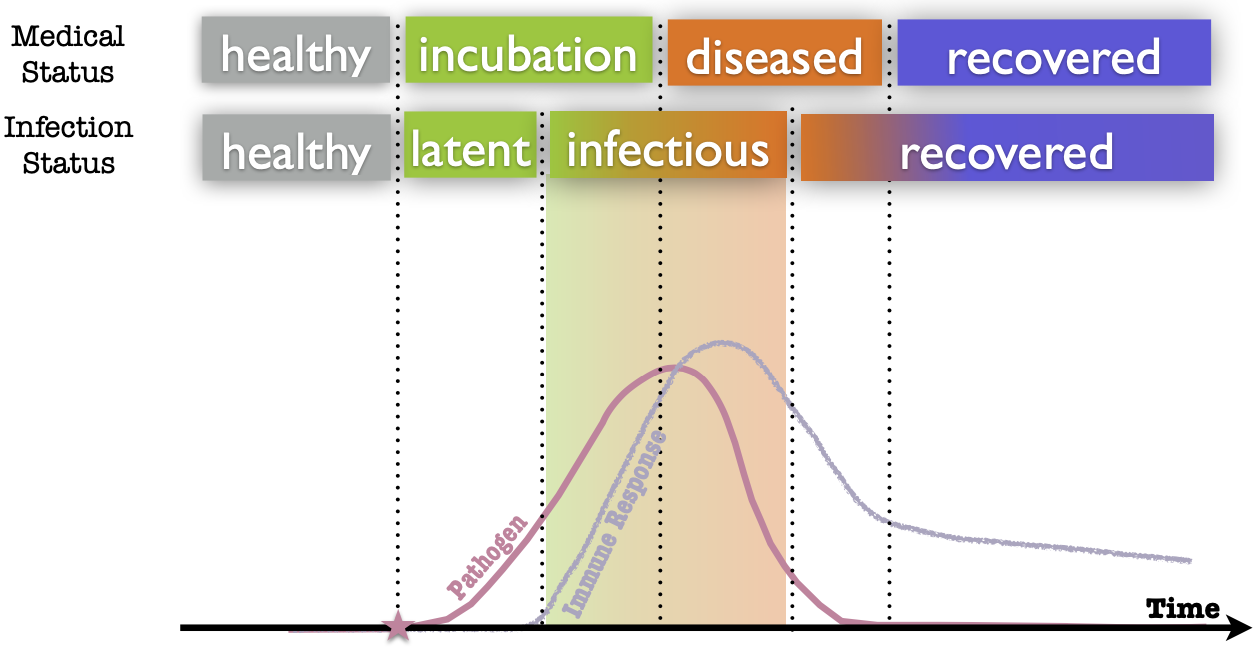
\includegraphics[width=0.7\textwidth]{../lessons/image/05/1.png}
\caption{\label{fig:05_1} Difference between infection status and medical status.}
\end{figure}

The transition of the SEIR model are:
\begin{equation}
\begin{split}
 S + I &\overset{\beta }{\rightarrow } I + E   \\
 E & \overset{\sigma }{\rightarrow } I  \\
 I & \overset{\mu }{\rightarrow } R
\end{split}
\end{equation}
with the equations:
\begin{equation}
  \begin{split}
    \dv{s}{t} &= \alpha -\beta s i - \alpha s \\
  \dv{i}{t} &= \beta s i - (\alpha + \sigma )e \\
  \dv{i}{t} &= \sigma e - (\alpha + \mu )i \\
  \dv{r}{t} &= \mu i - \alpha r
\end{split}
\end{equation}
Hence, the spreading is delayed due to the time in \( E \).

The \textbf{endemic state} is:
\begin{equation}
\begin{split}
s^*  &=  \frac{(\alpha +\mu )(\alpha + \sigma )}{\beta \sigma } = \frac{1}{R_0} \\
e^* &= \frac{\alpha (\alpha +\mu )}{\beta \sigma } (R_0 -1)\\
i^* &= \frac{\alpha }{\beta } (R_0 -1)
\end{split}
\end{equation}
For very short latent time (\( \sigma \rightarrow \infty  \)) we recover the endemic state of the SIR.

The \( R_0 \) factor is:
\begin{equation}
  R_0 = \frac{\beta \sigma }{(\alpha + \mu )(\alpha +\sigma )}
\end{equation}
Since latent time is way shorter than demography, usually \( \frac{\sigma }{\sigma + \alpha } \simeq 1 \) thus \( R_0 = \frac{\beta }{\alpha + \mu } \) as in the SIR with demography.

Since the endemic state, the infectious period and $R_0$ are similar between SEIR and SIR, adding exposed individuals it may seem an unnecessary complication but, if we look at the time evolution at the early stages there is a huge difference between SEIR and SIR model:
\begin{equation}
\begin{split}
  i_{SEIR} (t) & \approx e^{\qty(\sqrt{4(R_0-1)\sigma \mu  + (\sigma + \mu )^2} -(\sigma +\mu ))t/2 } \approx i_0 e^{\qty(\sqrt{R_0} -1 ) \mu t} \\
    i_{SIR} (t) &\approx i_0 e^{(R_0-1) \mu t}
\end{split}
\end{equation}
Even if the behavior at the steady state is similar the temporal evolution of SEIR is slower than SIR. This has important implications for policy making.

The SEIR can be the starting point for modeling realistic diseases: i.e. Covid-19 (see Fig. \ref{fig:05_2}).

\begin{figure}[h!]
\centering
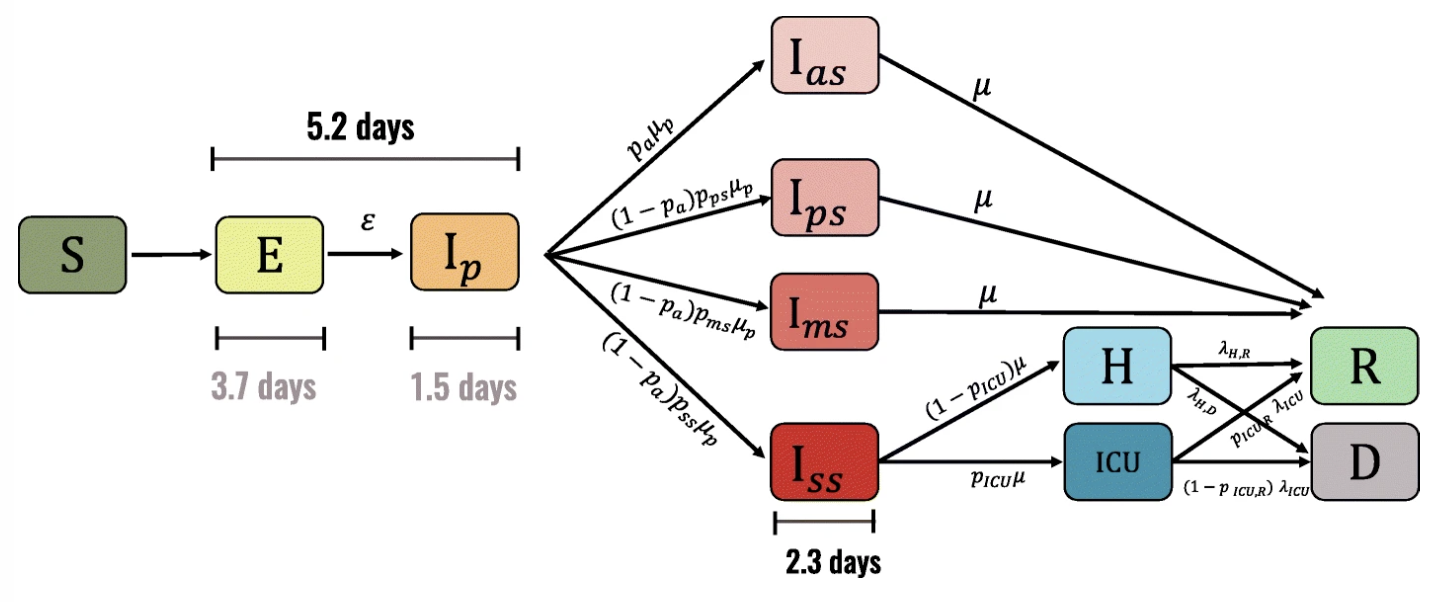
\includegraphics[width=0.7\textwidth]{../lessons/image/05/2.png}
\caption{\label{fig:05_2} Model for Covid-19.}
\end{figure}



\section{Summary of compartmental models in well-mixed populations}
Let us summarize all the comportmental models in well-mixed populations explained:
\begin{itemize}
\item we solved the \textbf{SI model} analitically and we observe that the growth is as a sigmoid:
\begin{equation*}
  i(t) = \frac{i_0 e^{\beta t} }{1-i_0 + i_0 e^{\beta t} }
\end{equation*}
In the early phases we have an exponential growth governed by \( \beta  \), and it always saturates at 1;

\item in the \textbf{SIS model} things starts to change. We have and endemic (meta-stable) state:
\begin{equation*}
  i= \frac{\beta -\mu }{\beta }
\end{equation*}
and we reach a sort of dynamic equlibrium. We can define an epidemic treshold:
\begin{equation*}
  \beta > \beta _c = \frac{\mu }{\expval{k} }
\end{equation*}

\item for the \textbf{SIR model} we cannot solve the equations analitically. We have no endemic state and the epidemic treshold is again:
\begin{equation*}
  \beta > \beta _c = \frac{\mu }{\expval{k} }
\end{equation*}

\item then, in the \textbf{SIRS model} we include waning immunity. This model interpolates between SIR and SIS model. We have the endemic state and the infectious period is:
\begin{equation*}
  \tau = \frac{1}{\alpha + \mu }
\end{equation*}
and moreover:
 \begin{equation*}
   R_0 = \frac{\beta }{\alpha + \mu }
 \end{equation*}

\item at the end, we have the \textbf{SEIR model} in which we include a latent period. We have that:
\begin{equation*}
  R_0 = \frac{\beta \sigma }{(\alpha + \mu )(\alpha +\sigma )}
\end{equation*}
and the exposed slow down the spreading.
\end{itemize}











\chapter{Basics of Network Science}

\section{Basics definition}

The most important thing is the concept of \textbf{network} (graph) \( G(V,E) \) which is just an object composed by a set of nodes (vertices) \( V \) and a set of links (edges) \( E \):
\begin{itemize}
\item the \textbf{nodes} represents the \emph{entities} \( V=[\dots,i,j,k,\dots] \) of the relationships, the entries, the people in a social network and so on. The number of nodes is \( N= \abs{V}  \);

\item the \textbf{links} represents the relationship between entities \( E=[\dots,(i,j),(i,k),\dots] \). The number of links is \( L= \abs{E}  \).
\end{itemize}

Links can be of different types and so networks: the basics distinction is between \textbf{undirected} and \textbf{directed} links.
Another important distinction is between \textbf{unweighted} and \textbf{weighted} links.

The \textbf{network density} (connectance) is the fraction of links over all the possible pairs:
\begin{equation}
  d = \frac{L}{N(N-1)}
\end{equation}
Real networks usually have a very low density, so are sparse systems (\( L \ll N^2 \)).

Another things that we will use a lot is the way of representing a graph in a mathematical sense. We will use the \textbf{adjacency matrix} \( A \) of the network, where:
\begin{itemize}
\item \( a_{ij} = 1 \), if a link between nodes \( i \) and \( j \) exists;
\item \( a_{ij} = 0 \) otherwise.
\end{itemize}
We can exploit many useful mathematical properties such as the spectrum of the matrix. Moreover, the matrix is symmetrical for undirected/unweighted graphs, i.e. \( a_{ij} = a_{ji} \).

Since real networks are usually sparse, the adjiacency matrix is inefficient for storing graphs in a computer, is better to use adjiacency lists, etc.

Two nodes that share a link are defined as connected, adjacent, neighbors. In particular, the \textbf{neighborhood} of node \( i \) is the set of nodes connected to \( i \).
The number of neighborhood \( k_i \) of each node \( i \) is what is called the \textbf{degree} of the node. This is the basic measure that we are gonna use a lot. Once you define the degree, the next step is defining what is the average of the degree over the entire network:
\begin{equation}
  \expval{k} = \frac{1}{N} \sum_{i=1}^{N} k_i, \qquad \text{or} \qquad \expval{k} = \frac{2L}{N} = d(N-1)
\end{equation}

The next definition is the concept of \textbf{path}, which is a sequence of links which permit to go from node \( i \) to node \( j \) following links.
Another important part is what is called the \textbf{shortest path} between \( i  \) and \( j \). This gives us the idea of how big the network is. In particular, the distance \( l_{ij} \) represents the length of the shortest path between \( i \) and \( j \). There could be multiple shortest paths between \( i \) and \( j \).

The network is \textbf{connected} if every possible couple of nodes is reachable trough a path. Otherwise, each connected part is defined as a connected \textbf{component}.


The shortest path of maximum length in the network is defined as \textbf{diameter}:
\begin{equation*}
  l_{max} = \max_{ij} l_{ij}
\end{equation*}
Another measure that is quite important is the \textbf{average (shortest) path length}:
\begin{equation*}
  \expval{I} = \frac{\sum_{ij}^{} l_{ij} }{N(N-1)}
\end{equation*}

Now, let us see some example as “The Oracle of Bacon”, the “Erdos Number” and so on.
The question which arises is: why such short distances in such large networks?
In particular, we note that in the last example of “Six degrees of separation” real networks are smaller (shorter) than one would expect.
This is what is called the small world phenomena. If you study the average path length which scales linearly as the scales of the network it scales as the logarithm of the network or in some case the logarithm of the logarithm of the network. This is huge important in the spreading of diseases.



\end{document}
